%
% Copyright (c) 2011-2012, fortiss GmbH.
% Licensed under the Apache License, Version 2.0.
% 
% Use, modification and distribution are subject to the terms specified
% in the accompanying license file LICENSE.txt located at the root directory
% of this software distribution. A copy is available at
% http://chromosome.fortiss.org/.
%
% This file is part of CHROMOSOME.
%
% $Id$
%
% Author:
%         Dominik Sojer <sojer@fortiss.org>
%         Michael Geisinger <geisinger@fortiss.org>
%

\section{\xme in a Nutshell (30 minutes)} \label{sec:architecture}

\xme (often abbreviated by ``XME'') is a domain-independent, data-centric\footnote{%
For details, please refer to \url{http://www.omg.org/news/whitepapers/Intro_To_DDS.pdf}}
middleware for cyber-physical systems.
%
From the point of view of an application component,
\xme abstracts from basic functionality that is traditionally found in operating systems and middlewares,
like scheduling and communication.
%
This section will give the reader a very high level overview of the most important \xme features.
For in-depth information and concrete specifications, the reader is kindly referred to the commented source code of \xme.

\subsection{Goals of \xme}
\xme is designed to match the requirements of future cyber-physical systems.
As a research prototype, the main intention is to serve as a basis
for discussion how future middleware/operating system architectures may look like.
The development is done in a demand-driven way.
Depending on the requirements of projects where \xme is applied, new features in \xme will be introduced.

The current version is the first version of \xme and therefore provides only very basic funcitonality.
Further features will be introduced in the future. In the following, the main concepts of \xme are introduced.
In addition, we state whether these features are already implemented or planned for future versions.
%In the following, the goals of \xme and major concepts to achieve these goals are listed.
%
%\subsubsection{Scalability \& Modularity}
%
Our point of view is that
future middleware will not operate on a specific class of devices, but will run on very heterogeneous platforms.
The exaggerated goal statement could be to ``develop a middleware serving a range from 8-bit controllers to cloud servers''.

Therefore, scalability and modularity of the middleware is of highest importance. It must be easy to remove or add components from/to 
the middleware. Similar to micro-kernel operating systems, the core of \xme must be very small and only contain the absolutely necessary
features. Since the boundaries of operating systems, middleware, and applications are vanishing, one unique mechanism must be supported to
add components on all these levels.

\paragraph{Concept 1: Data-Centric Design} A very succesful concept to achieve scalability is message-orientation as for example demonstrated
by the QNX\footnote{\url{http://www.qnx.com/}} neutrino micro-kernel.
However, one major drawback of this concept is the necessity of requiring knowledge of both the sender and the receiver.
In the context of systems-of-systems where the communication partners are not known at design time, message orientation cannot be applied.
Therefore, \xme is based on the very powerful concept of data-centric design. Components specify which data they consume
and produce and based on this information, the middleware calculates the communication routes.

It is important to note that in contrast to prominent other middleware systems relying on data-centric design,
\xme does not broadcast the data, instead it calculates specific routes based on the requirements.
This allows for a very efficient implementation. Furthermore, the routes are calculated only when components are added or removed. Based
on the experience in embedded systems, we assume that reconfiguration takes places less often than the transmission of data items.
Similar to concepts from multimedia protocols,
our initial assumption is that data transmission has to happen within real-time,
while reconfiguration is not time-critical or has only soft real-time requirements.

Data is grouped by so-called \emph{topics}. A topic is a data type with a certain structure.
Examples for topics are temperature or rotation speed. Topics are defined for a specific domain.
This enables the exchange of data between different applications.
To allow cross-domain communication, we plan to define translation matrixes between the topics of different domains.

\paragraph{Concept 2: Meta-Data Support (not yet implemented)}
	Exchange of data can only be automated if the requirements on data are specified explicitly.
	This includes information about the quality of data such as age, accuracy, confidence, and safety level.
	In the future, we plan to support respective annotations to data, so-called \emph{meta-data}, to specify these requirements.
	
	Using meta-data, application components describe their requirements respectively guarantees on data.
	This information can be used to select appropriate communication streams while still retaining independence between sender and receiver.
	
	We are planning to support two scenarios:
	\begin{itemize}
		\item \textbf{Static meta-data:}
			Application components have fixed requirements and guarantees.
			Meta-data are used to calculate the appropriate communication routes at configuration time.
			For example, imagine a temperature sensor network for building automation.
			Depending on its size, multiple sensors may be present in a room.
			Each sensor would specify its \emph{location} as meta-data.
			A climate control component that controls the air conditioning system for a specific room would specify, using meta-data,
			that it only wants to receive temperature data from sensors that match the respective room.
		
		\item \textbf{Dynamic meta-data:}
			Application components producing data may specify meta-data such as the quality of the transmitted values dynamically during runtime.
			Consuming components may have dynamic meta-data acceptance filters and may use meta-data also for their calculations.
			For example, imagine that one of the rooms in the auotmated building from the previous example is a server room.
			In this case, a high reliability is required.
			Using meta-data about the confidence of each sensor,
			the climate control may dynamically calculate the confidence in its own set value for the air conditioning system.
			The association of data from the respective room could still use static meta-data.
	\end{itemize}

\paragraph{Concept 3: Data Access}
Components can access data in two different ways. As standard operation, \xme provides a publish-subscribe mechanism. Each component states
which data is required and which data is produced. The middleware ensures the routing of the specific data. If data is only required 
seldomly in comparison to the data production rate, a request-response mechanism is offered to the application developer.

\paragraph{Concept 4: Timing (not yet implemented)}
Correct timing is a major concern for cyber-physical systems. \xme abstracts the concrete implementation, but will offer mechanisms to
specify end-to-end-timing and jitter requirements for data paths.
The reason to abstract the concrete implementation / concrete configuration
in \xme is on the one hand to reduce the development effort by automatically deriving a concrete configuration satisfying the timing
requirements (if a configuration exists) and on the other hand to support plug~\&~play capability. The state of the art in embedded system
design requires the developer to configure the application in a correct way. Several configurations might be valid, but typically only one
configuration is specified. It is not possible for the run-time system to change the configuration, as the real requirements are not present
any more and the system can not calculate alternative configurations. By explicitly stating the requirements and leaving configuration issues
to the run-time system, this problem can be avoided.
The system can support new components by calculating a new configuration that satisfies both
the requirements of already running applications and the newly installed applications.

It is important to note that \xme can of course only offer guarantees that are enabled by the underlying platform.
In case \xme runs on Windows, \xme will not be able to satisfy jitter requirements in the range of microseconds.
Nevertheless, different implementations of components will offer very good guarantees.
The major concept here is to use algorithms that offer determinism sacrificing average-case performance.
Examples are the implementation of a time-triggered communication scheme on top of Ethernet.
This implementation guarantees collision free communication, but comes with a lower bandwidth and flexibility.

\paragraph{Concept 5: Resource-Awareness (not yet implemented)}
\xme is designed to be able to handle all resources of the platform.
The major idea is that components / applications can state their worst-case resource requirements
on memory, computation time, bandwidth, etc.
\xme will then ensure that enough resources are available to allow the execution of this component / application.

\paragraph{Concept 6: Other extra-functional properties -- Fault-tolerance, QoS, Security (not yet implemented)}
\xme is designed in a way such that components which guarantee other extra-functional properties can be easily extended.
Examples on extra-functional properties that are currently being integrated in \xme are fault-tolerance, QoS, and security.

\paragraph{Concept 7: Support for States (not yet implemented)}
A very important topic to ensure resource efficiency is state awareness.
We are currently thinking about possibilities to support states
(each one with a set of active applications) in \xme.
The support of (sub-)system wide states would simplify the development of applications,
but also other aspects such as fault-tolerance.

\begin{figure}[htb]
	\centering
	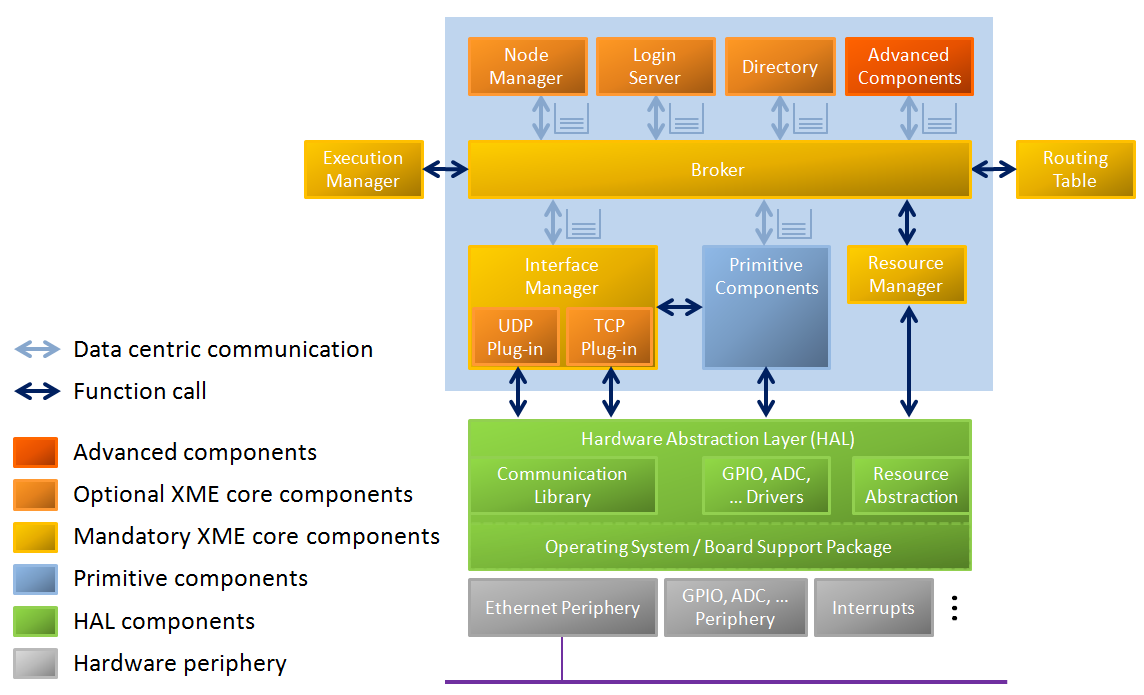
\includegraphics[width=\textwidth]{figures/PNG/architecture.png}
	\caption{\xme architecture overview.}
	\label{fig:architecture}
\end{figure}

\subsection{Core Components}
\label{sec:core_components}
\xme is designed in a modular fashion. Its component-oriented architecture is depicted in Figure~\ref{fig:architecture}.
A (distributed) \emph{application} consists of a set of (software) \emph{components} that interact with each other by exchanging data.
Each component is placed on a specific \emph{node} in the network.
On operating system based platforms like Windows,
the software of a node is typically represented by a console application.
On embedded systems, the software of a node corresponds to the firmware.
%
The following sections provide brief descriptions of the most important core components of \xme.
See Figure~\ref{fig:architecture} for a graphical illustration.

\subsubsection{Node Manager}

A node can have an arbitrary amount of software components that implement the application.
The \emph{Node Manager} is responsible for connecting a new node to the network and obtaining a so-called \emph{node identifier}.
The node identifier is a unique address of the node within a network.
The Node Manager periodically tries to obtain such a node identifier from the \emph{Login Server},
which is present on one specific node in the network.

\subsubsection{Login Server}

The \emph{Login Server} maintains a list of all nodes in the \xme network.
It receives login requests from the Node Managers of all other nodes and handles them accordingly.
Only one Login Server should exist in the network.

\subsubsection{Directory}

The \emph{Directory} maintains a list (a directory, as the name implies)
of all publication and subscription requests in the network
and is responsible for root calculation and setup.
Usually, only one so-called \emph{Master} Directory exists in the network, which is the autority for route calculation.
All other nodes have a so-called \emph{Local} Directory, which is only authoritative for local routes
and forwards announcements (publication and subscription requests) to the Master Directory.
Setup of routes is performed by modifying the \emph{Routing Tables} present on every node.

\subsubsection{Routing Table}

As the name implies, the \emph{Routing Table} is a data structure that contains routing information.
In \xme, routing is performed via so-called \emph{data channels}.
A data channel is a system-internal identifier for a communication path.
When data arrive at a node, the Routing Table is inspected to determine where the data has to be delivered to.
This is done by the \emph{Broker}.

\subsubsection{Broker}

The \emph{Broker} is response for delivering incoming data to the correct destination,
which can be determined from the Routing Table.
The Broker is also responsible for buffering the data if it can not be delivered immediately.
The decision of when data can be delivered to a component is issued by the \textit{Execution Manager}.

\subsubsection{Execution Manager}

The \emph{Execution Manager} is the facility that enforces the model of execution in the system
(according to a schedule).
It determines when tasks are executed and when incoming data are processed by components.
Data that are not immediately processed are put into queues.

\subsubsection{Resource Manager}

The \emph{Resource Manager} is the node-local authority for resource reservation and arbitration.
Among others, managed resources include memory and CPU time.
Components report their requirements to the directory and only get them assigned when enough resources are available.

\subsubsection{Interface Manager}

The \emph{Interface Manager} abstracts from the communication interfaces available at a certain node.
Typical submodules of the Interface Manager are facilities for communication over Ethernet/IP with UDP or TCP.
When data is to be sent, it is delivered from the Broker to the Interface Manager.
Incoming data from the network is forwarded to the Broker to decide where to deliver it to.

\subsubsection{Primitive Components}

\emph{Primitive Components} directly access the \emph{Hardware Abstract Layer} using function calls
and offer data obtained from the hardware in a data centric way or forward data to the respective actuators.
They are typically the source of physical data obtained from the environment and
the sink for control data to the environment.

\subsubsection{Hardware Abstraction Layer}

The \emph{Hardware Abstraction Layer}, often abbreviated by HAL,
provides a platform indepdent application programming interface (API).
\xme components are implemented against that API and hence are platform independent.
The HAL typically implements hardware-specific functionality such as drivers for microcontroller periphery
like general purpose I/O (GPIO) or analog to digital conversion (ADC).

\subsubsection{Advanced Components}

The actual (distributed) application running in the network is implemented by application-specific \emph{Advanced Components}.
Advanced Components operate solely on data obtained via data centric communication.
In particular, no direct access to the Hardware Abstraction Layer with effects in the environment is allowed.

\subsubsection{Login Client Proxy and IP Login Server Proxy}

These components are required for new nodes to initially contact the Login Server.
A node that does not have a Login Server will usually have a \emph{Login Server Proxy} component for each of its physical network interfaces.
These components are named according to their associated interface types,
for example \emph{IP Login Server Proxy} for an Ethernet interface with IP communication stack.
Whenever the Node Manager, which is responsible for periodic login requests, issues a login request,
the Login Server Proxy takes care of broadcasting it over its associated communication interface.

Nodes that have a Login Server component usually also have a \emph{Login Client Proxy} for each of their interfaces.
The Login Client Proxy will receive the login requests issued by the Login Server Proxy on the respective medium
and forward them locally to the Login Server.
The login response is forwarded in a similar manner.
%
This concept makes it possible to separate the login and address assignment logic from specific interface types and communication protocols
and enables a fine-grained assignment of functionality to each communication interface.

\subsection{Component Definition and Lifecycle}
\label{sec:component_definition}

\xme components are assigned to one of the following categories according to their ``layer'' within the system:
\verb|adv| (advanced), \verb|prim| (primitive), \verb|core| (runtime system) or \verb|hal| (hardware abstraction).
A \xme component is defined by four functions to \emph{create}, \emph{activate}, \emph{deactivate} and \emph{destroy} it,
illustrated here for a component called \verb|xme_adv_myComponent|:
\begin{quote}
	%\verb|xme_core_status_t|\\
	\verb|xme_adv_myComponent_create(xme_adv_myComponent_configStruct_t*);|\\
	%\verb|xme_core_status_t|\\
	\verb|xme_adv_myComponent_activate(xme_adv_myComponent_configStruct_t*);|\\
	%\verb|void|\\
	\verb|xme_adv_myComponent_deactivate(xme_adv_myComponent_configStruct_t*);|\\
	%\verb|void|\\
	\verb|xme_adv_myComponent_destroy(xme_adv_myComponent_configStruct_t*);|
\end{quote}
%
The distinction between creation/activation and deactivation/destruction is required in case a component needs to be migrated:
in this case, the component is first deactivated (to obtain a consistent state), then moved and activated at the new location.
All four functions take a pointer to a configuration structure, which represents the state of the respective component instance.
Multiple component instances of the same component type usually have their own configuration structures.

A typical task during creation of a component is registration of data demand and data production.
Furthermore, a component may create (periodic) tasks to implement its functionality.
These two concepts are illustrated in the following sections.

\subsection{Component Instantiation}

Components can be instantiated by adding them to the so-called \emph{component list}, usually defined in the main program file.
Mandatory core components (compare Figure~\ref{fig:architecture}) are implicitly added to the list.
An initial configuration may be provided for each component.
Listing~\ref{lst:component_list} shows a sample component list with respective configurations.

\begin{lstlisting}[numbers=left,float=htpb,label=lst:component_list,caption=Sample component list with component configurations.]
/*****************************************************************************/
/***   Component configurations                                            ***/
/*****************************************************************************/
XME_COMPONENT_CONFIG_INSTANCE(xme_core_nodeManager) = ~\label{lst:component_list.initialized_config_begin}~
{
	0x00000000021041A1, // deviceType
	XME_CORE_DEVICE_GUID_RANDOM // deviceGuid
}; ~\label{lst:component_list.initialized_config_end}~

XME_COMPONENT_CONFIG_INSTANCE(xme_prim_ipLoginServerProxy, 1); ~\label{lst:component_list.uninitialized_config}~

/*****************************************************************************/
/***   Component descriptor                                                ***/
/*****************************************************************************/
XME_COMPONENT_LIST_BEGIN
	XME_COMPONENT_LIST_ITEM(xme_core_nodeManager, 0) ~\label{lst:component_list.stateful_1}~
	XME_COMPONENT_LIST_ITEM(xme_prim_ipLoginServerProxy, 0) ~\label{lst:component_list.stateful_2}~
	XME_COMPONENT_LIST_ITEM_NO_CONFIG(xme_adv_myComponent) ~\label{lst:component_list.stateless}~
XME_COMPONENT_LIST_END;
\end{lstlisting}

This example declares that three components (besides internal core components),
namely \verb|xme_core_nodeManager|, \verb|xme_prim_ipLoginServerProxy| and \verb|xme_adv_myComponent|,
will be present on this node.
We can distinguish between the following types of components:
\begin{enumerate}
	\item \textbf{Components with internal state:}
		The \verb|XME_COMPONENT_LIST_ITEM()| macro is used to declare such a component
		(compare lines~\ref{lst:component_list.stateful_1} and~\ref{lst:component_list.stateful_2}).
		The second parameter of the macro is the zero-based index of the respective configuration
		(defined above the list) that is used to initialize the component.
		
		Some components expect some of their configuration variables to be initialized properly.
		For example, the \emph{Node Manager} expects its \emph{device type} and \emph{device GUID}
		members to be set up.
		This is achived by assigning values to the respective members
		when declaring the configuration structure with the \verb|XME_COMPONENT_CONFIG_INSTANCE| macro
		(compare lines~\ref{lst:component_list.initialized_config_begin}--\ref{lst:component_list.initialized_config_end}).
		Configurations for multiple components of the same type can be declared
		by separating multiple initialization blocks with commas and using the respective index in the
		\verb|XME_COMPONENT_LIST_ITEM()| macro.
		
		Other components, like the \emph{IP Login Server Proxy}, do not require any special configuration.
		They only need a properly defined configuration structure to store their state during runtime.
		Again, the \verb|XME_COMPONENT_CONFIG_INSTANCE| macro is used
		with the second parameter set to the number of configuration structures for that component type to create
		(we could also declare multiple components of the same type), in this case one
		(line~\ref{lst:component_list.uninitialized_config}).
	
	\item \textbf{Components without internal state:}
		The \verb|XME_COMPONENT_LIST_ITEM_NO_CONFIG()| macro is used to declare such a component
		(compare line~\ref{lst:component_list.stateless}).
		In this case, \verb|NULL| will be passed in the \verb|config| parameters of the four functions introduced in Section~\ref{sec:component_definition}.
\end{enumerate}

The list item macro calls have to be embedded between the \verb|XME_COMPONENT_LIST_BEGIN| and \verb|XME_COMPONENT_LIST_END| macro calls.
%
Components declared in this list are automatically created and activated during startup
and deactivated and destroyed during shutdown.

\subsection{Sending and Receiving Data}

Before sending data, a component states its intent to the runtime system.
This is necessary to allow the appropriate communication routes to be set up
and is usually performed from within a component's \emph{create} function.
%
For using data centric communication, \verb|#include| the file \verb|"xme/core/dcc.h"|.
%
To inform \xme that a component intends to send data under a specific \verb|topic|, call:
\begin{quote}
	\verb|publicationHandle =|\\
	\verb|    xme_core_dcc_publishTopic(|\\
	\verb|        topic, XME_CORE_MD_EMPTY_META_DATA, NULL|\\
	\verb|    );|
\end{quote}

The actual sending of \verb|data| is performed with:
\begin{quote}
	\verb|xme_core_dcc_sendTopicData(|\\
	\verb|    publicationHandle, &data, sizeof(data)|\\
	\verb|);|
\end{quote}

A component can subscribe to a certain \verb|topic| with a given \verb|receiveTopicCallback| function by calling:
\begin{quote}
	\verb|subscriptionHandle =|\\
	\verb|    xme_core_dcc_subscribeTopic(|\\
	\verb|        topic, XME_CORE_MD_EMPTY_META_DATA, receiveTopicCallback, NULL|\\
	\verb|    );|
\end{quote}
Whenever data matching the given topic is received, the given callback function is invoked.
The last parameter of the function can be used to pass user-defined data to the callback function,
for example a pointer to the component's configuration structure.
%
\verb|receiveTopicCallback| must have a signature matching \verb|xme_core_dcc_receiveTopicCallback_t|, namely:
\begin{quote}
	\verb|void receiveTopicCallback(xme_hal_sharedPtr_t dataHandle, void* userData);|
\end{quote}
\verb|dataHandle| is a reference to the memory where the received data is located.

\subsection{Working with Tasks}

Tasks are allocated via the resource manager,
hence \verb|#include| \verb|"xme/core/resourceManager.h"| to use them.
A component can create one or multiple asynchronous tasks by calling

\begin{quote}
	\verb|taskHandle = |\\
	\verb|    xme_core_resourceManager_scheduleTask(|\\
	\verb|        startMs, periodMs, XME_HAL_SCHED_PRIORITY_NORMAL,|\\
	\verb|        taskCallback, NULL|\\
	\verb|    );|
\end{quote}

This function registers the \verb|taskCallback| function to be scheduled for execution
according to \verb|startMs| (number of milliseconds before first invocation) and
\verb|periodMs| (interval between invocations).
%
The last parameter of the function can be used to pass user-defined data to the callback function,
for example a pointer to the component's configuration structure.
%
\verb|taskCallback| must have a signature matching \verb|xme_hal_sched_taskCallback_t|, namely:
\begin{quote}
	\verb|void taskCallback(void* userData);|
\end{quote}

A task can be suspended or resumed by calling:

\begin{quote}
	\verb|xme_hal_sched_setTaskExecutionState(|\\
	\verb|    taskHandle, <flag>|\\
	\verb|);|
\end{quote}

\verb|<flag>| is a Boolean flag that indicates the new task execution state.
The call will block until the new state can be enforced,
which is not the case while the task's callback function is executed.
%A task's callback function should return periodically
%and the \verb|periodMs| argument in the \verb|xme_core_resourceManager_scheduleTask()| call
%should be used to reschedule themselves at the appropriate points in time.
%
A task can be aborted by calling:

\begin{quote}
	\verb|xme_core_resourceManager_killTask(|\\
	\verb|    taskHandle|\\
	\verb|);|
\end{quote}

If this function is called from the task to kill itself, then it will mark the task for deletion and return immediately.
If it is called from a different task, the function blocks until the task has been removed.
Similarly to suspension and resuming, a task is not removed until its callback function has returned.
